\documentclass{article}
\usepackage[utf8]{inputenc}
\usepackage{graphicx}

\title{CHAPTER 2}
\author{John Kevin Giraldi (1184049) }
\date{7 October 2019}

\begin{document}

\maketitle

\section{TEORI}
\subsection{Variable}
\paragraph{Penjelasan mengenai variabel dalam dunia pemrograman adalah identitas yang digunakan untuk menampung suatu nilai. Nilai tersebut dapat berubah-ubah tergantung dengan keperluan program.
\par
Dapat dikatakan juga bahwa variabel ini seperti tempat penyimpanan yang bisa diisi dengan berbagai data dan (posisi) tempat tersebut bisa kita pindah-pindah sesuai keperluan.
\par
Secara teknis, variabel merujuk kepada suatu alamat di memory komputer. Setiap variabel memiliki nama yang digunakan sebagai identitas untuk menjangkau variabel tersebut.}

\begin{itemize}
    \item Jenis-jenis variabel antara lain :
    \begin{enumerate}
        \item Bilangan bulat (integer)
        \item String (character)
        \item Notasi matematika (float)
    \end{enumerate}
    \item Contoh penggunaan variable pada Python :
    
\begin{figure}[ht]
	\centering
	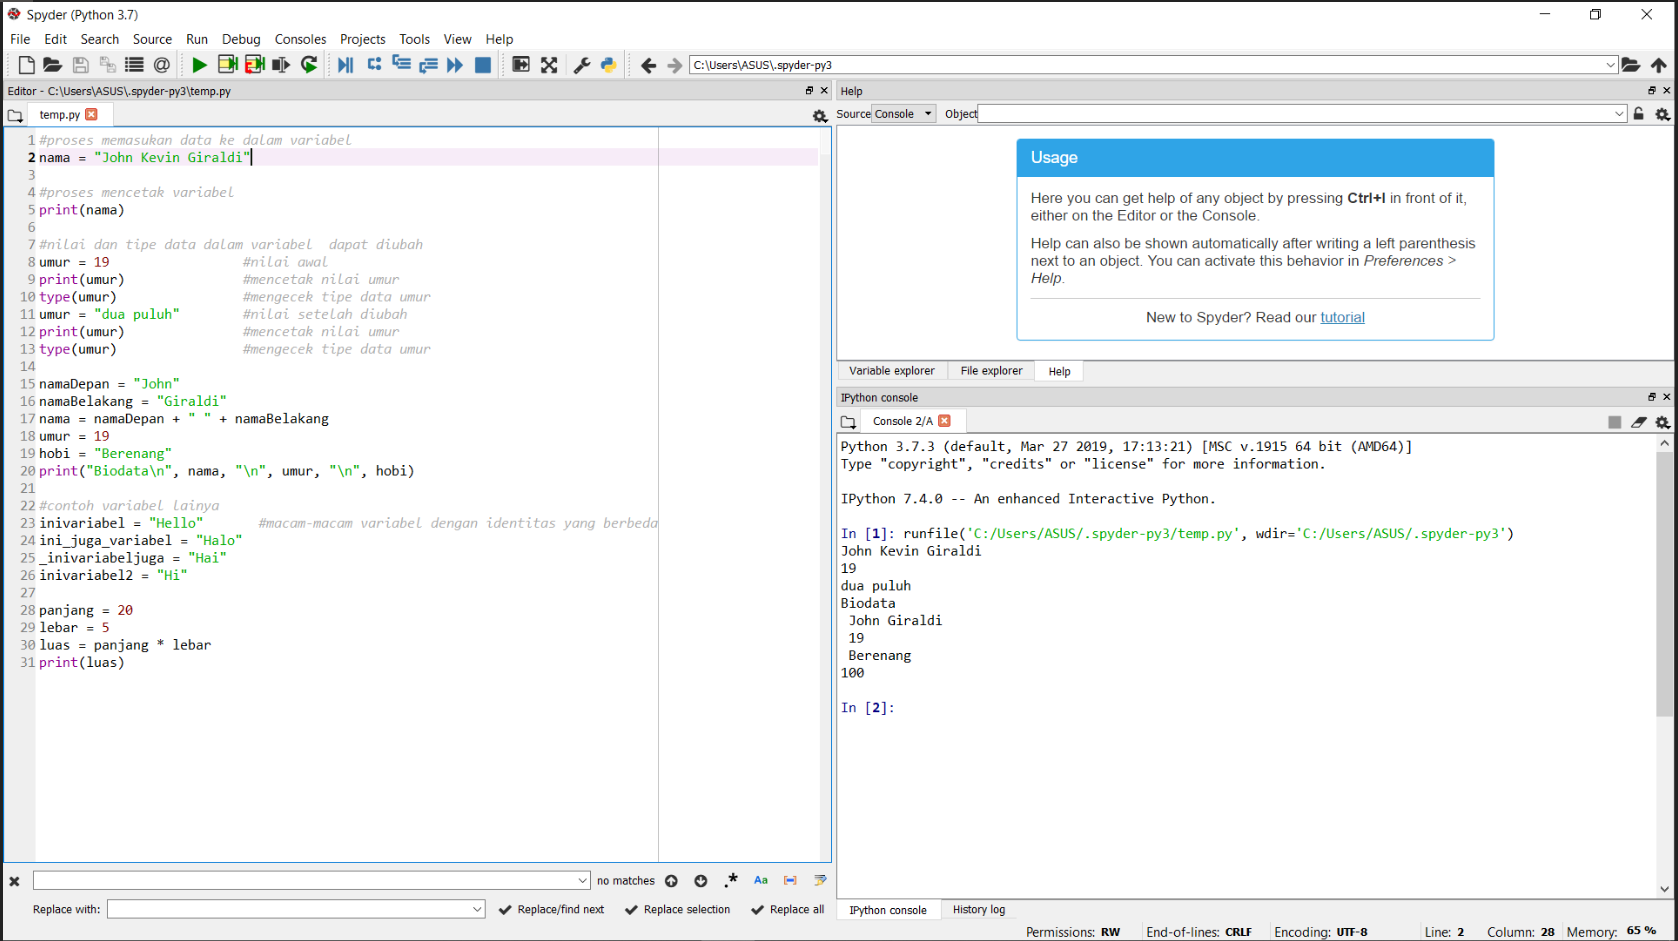
\includegraphics[width=6.5cm]{figures/cv.PNG}
	\end{figure}
\end{itemize}

\subsection{Input dan Output User}
\begin{itemize}
    \item Input menggunakan fungsi input ()
    \item Pada Python 3, Anda memiliki input ().
    \item Pada Python 2, Anda memiliki fungsi built\textunderscore in raw\textunderscore input ()
    \item Python memiliki fungsi input yang memungkinkan Anda meminta input teks kepada pengguna. Anda memanggil fungsi ini untuk memberi tahu program untuk berhenti dan menunggu pengguna memasukkan data
\end{itemize}

\subsection{Operator 2}
\subsubsection{Operasi Aritmatika}
\begin{table}[h]
    \centering
\begin{tabular}{|c|c|}
\hline
Operator & Simbol\\
\hline
Pembagian & /\\
\hline
Perkalian & *\\
\hline
Penjumlahan & +\\
\hline
Pengurangan & -\\
\hline
Modulus & \% \\
\hline
Pangkat & **\\
\hline
\end{tabular}
\end{table}\\
Cara mengubah variabel integer ke string :
\par
a = 100
string = str(a)
print(string)

\paragraph{}
Operasi matematika sebagai bahasa pemrograman, Python memiliki operasi aritmatika seperti tambah, kurang, kali, bagi. Berikut adalah contoh penggunaan operasi aritmatika pada python
Contoh misalnya kita mempunyai variable : a=2 dan b=4\\

\subsubsection{Casting}
\paragraph{}
Lalu apa yang akan terjadi bila ternyata variabel a adalah string dan variabel b adalah integer, contoh a=”6” dan b=4, tentunya program akan error bukan? Disinilah casting digunakan. Casting adalah cara untuk mengubah tipe data dari suatu data primitive, Jadi misal kita akan menjumlahkan variabel a dan b seperti contoh diatas tetapi logikanya sebuah kata (string) tidak akan bisa dijumlahkan dengan angka (“6” + 4) karena variabel a diapit oleh tanda kutip, ini berarti variabel a bertipe data string untuk itu kita perlu merubah dulu variabel a yang tadinya string menjadi integer. Berikut adalah sintax untuk melakukan casting :
\begin{itemize}
	\item int(var/value) : mengubah tipe data ke integer, contoh int(angka)
	\item float(var/value) : mengubah tipe data ke float, contoh float(hasil)
	\item string(var/value) : mengubah tipe data ke str, contoh string(12)
\end{itemize}
Mengubah string ke integer : type data string harus dilakukan casting dengan "int(variable)".
Mengubah integer ke string : type data integer harus dilakukan casting dengan "str(variable)".\\

\subsection{Syntax Perulangan}

\item Di dalam bahasa pemrograman Python pengulangan dibagi menjadi 3 bagian

\begin{itemize}
    \item While Loop\\
While : untuk melakukan looping yang tidak pasti\\
Contoh :\\
i = 0\\
While True :\\
    if i \textless 100:\\
        print ("i bernilai : "), i\\
        i = i + 1\\
    elif i \textgreater = 100:\\
        break\\
    \item For Loop\\
For : Melakukan looping yang sudah pasti jumlahnya\\
Contoh :\\
for i in range(0, 100):\\
    print (i)\\
    \item Nested Loop\\
Bahasa pemrograman Python memungkinkan penggunaan satu lingkaran di dalam loop lain. Dibawah ini menunjukkan beberapa contoh untuk menggambarkan konsep tersebut \\
Contoh penggunaan Nested Loop

i = 2\\
while(i \textless 50):\\
    j = 2\\
    while(j \textless= (i/j)):\\
        if not(i%j): break\\
        j = j + 1\\
    if (j \textgreater i/j) : print(i, "is prime")\\
    i = i + 1\\
print "Good bye!"
\end{itemize}

    \subsection {Syntax Kondisi}\\
    \textbf{Struktur if}
    \item Sederhananya struktuf if dalam Python dijalankan untuk mengecek kondisi ini bernilai benar atau salah. Apabila kondisi  bernilai benar, maka python akan menjalankan statement dalam blok kondisi tersebut dan sebaliknya jika kondisi bernilai salah maka statement dalam blok tersebut tidak akan dijalankan.\\
    
    \textbf{Struktur if – else}
    \item Struktur if sebelumnya hanya menjalankan statement dalam blok kondisi jika bernilai benar, maka struktur if-else adalah membuat statement kondisi yang bernilai benar dan salah.


\item If : digunakan untuk percabangan\\
Contoh :\\
umur = 20\\
if umur \textgreater 17:\\
    print("Remaja")\\
\item Else\\
Else : jika kondisi if tidak terpenuhi maka dijalankan kondisi else\\
Contoh :\\
umur = 6\\
if umur \textgreater 17:\\
    print ("beranjak dewasa")\\
else:\\
    print ("anak-anak")\\

\subsection{Try & Except}\\
\textbf{Menangani Eksepsi Menggunakan Try, Except, dan Finally}\\

Terjadinya eksepsi pada suatu program bisa membuat program berhenti. Untuk mencegahnya, Maka kita harus mengantisipasi hal tersebut.

Python menyediakan metode penanganan eksepsi dengan menggunakan pernyataan \textit{try dan except}.

Dalam blok try kita akan meletakkan baris program yang mungkin akan terjadi error. Apabila terjadi error, maka cara penanganannya diserahkan kepada blok except. \\

\textbf{contoh try…finally untuk mengoperasikan file.} 
try:\\
    f = open("C:test.txt")\\
    # melakukan operasi terhadap file\\
finally:\\
    f.close()\\
\end{document}